\documentclass[usenames,dvipsnames,aspectratio=169]{beamer}
\usepackage{../common/prgBasics}

\title[Lecture 4.]{Programming basics}
\subtitle{(GKNB\_INTA023)}

\begin{document}

%1
\begin{frame}[plain]
  \titlepage
  \logoalul
\end{frame}

%2
\begin{frame}{Triangle equality}
  \begin{exampleblock}{\textattachfile{triangle1.c}{triangle1.c} ANSI C (C89) compliant implementation}
  \tiny
  \vspace{-.3cm}
  \lstinputlisting[style=c]{triangle1.c}
  \vspace{-.3cm}
  \end{exampleblock}
\end{frame}

%3
\begin{frame}{Triangle equality}
  \footnotesize
  \begin{exampleblock}{\textattachfile{triangle2.c}{triangle2.c} C99 compliant implementation; reading side lengths are repeated 3x!}
  \tiny
  \vspace{-.3cm}
  \lstinputlisting[style=c]{triangle2.c}
  \vspace{-.3cm}
  \end{exampleblock}
\end{frame}

%4
\begin{frame}{Triangle equality}
  \begin{exampleblock}{\textattachfile{triangle3.c}{triangle3.c}}
    \tiny
    \vspace{-.3cm}
    \lstinputlisting[style=c]{triangle3.c}
    \vspace{-.3cm}
  \end{exampleblock}
\end{frame}

%5
\begin{frame}[fragile]{Triangle equality}
  Array definition
  \begin{itemize}
    \item \emph{type name[size];}
    \item eg. \texttt{int sideArray[3];}
    \item \emph{size} is a positive integer valued \emph{constant expression}
    \item the the value of a \emph{constant expression} can be calculated compile-time
  \end{itemize}
  Memory requirement of an array
  \begin{itemize}
    \item[] \emph{sizeof(name\_of\_the\_array) $\equiv$ size*sizeof(type)}
  \end{itemize}
  Accessing array elements
  \begin{itemize}
    \item \emph{name[index]}
    \item 0 $\leq$ \emph{index} $\leq$ \emph{size}$-$1
  \end{itemize}
  \hspace{4mm}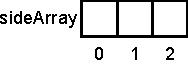
\includegraphics[]{array.pdf}
\end{frame}

%6
\begin{frame}{Triangle equality}
    \begin{exampleblock}{\textattachfile{triangle4.c}{triangle4.c}}
    \tiny
    \vspace{-.3cm}
    \lstinputlisting[style=c]{triangle4.c}
    \vspace{-.3cm}
  \end{exampleblock}
\end{frame}

%7
\begin{frame}[fragile]{Triangle equality}
  Generating side names
  \begin{itemize}
    \item ASCII codes of letters in ascending order are also increasing \\ ('A' == 65, 'B' == 66, 
\dots, 'Z' == 90)
    \item Digits are encoded similarly ('0' == 48, '1' == 49, \dots, '9' == 57)
    \item Digit $\rightarrow$ ASCII code: \texttt{'0'+digit}
    \item ASCII code $\rightarrow$ digit: \texttt{character-'0'}
    \item Letters can be handled similarly
  \end{itemize}
  \begin{exampleblock}{}
    \tiny
    \lstinputlisting[style=c,linerange={14-14},firstnumber=14]{triangle4.c}
  \end{exampleblock}
  Format specifier: \kiemel{\texttt{\%c}} (single character, not terminated by zero!)\\
  Character literals are between apostrophes!
\end{frame}

%8
\begin{frame}{Counting digits}
    \begin{exampleblock}{\textattachfile{counter1.c}{counter1.c} 1/2}
    \tiny
    \lstinputlisting[style=c,lastline=23]{counter1.c}
  \end{exampleblock}
\end{frame}

%9
\begin{frame}{Counting digits}
    \begin{exampleblock}{\textattachfile{counter1.c}{counter1.c} 2/2}
    \scriptsize
    \lstinputlisting[style=c,firstline=24,firstnumber=24]{counter1.c}
  \end{exampleblock}
  \vfill
  We urgently need an array!
\end{frame}

%10
\begin{frame}{Counting digits}
    \begin{exampleblock}{\textattachfile{counter2.c}{counter2.c} 1/2}
    \footnotesize
    \lstinputlisting[style=c,lastline=13]{counter2.c}
  \end{exampleblock}
\end{frame}

%11
\begin{frame}{Counting digits}
    \begin{exampleblock}{\textattachfile{counter2.c}{counter2.c} 2/2}
    \scriptsize
    \lstinputlisting[style=c,firstline=14,firstnumber=15]{counter2.c}
  \end{exampleblock}
\end{frame}

%12
\begin{frame}{Counting digits}
  Array elements as counters
  \begin{itemize}
    \item[] The number of digit \kiemel{i} is stored at \kiemel{digits[i]} (eg. 0 $\to$ digits[0], 1 $\to$ digits[1], etc.)
  \end{itemize}
  \vfill
  Initialization of arrays
  \begin{itemize}
    \item \emph{type name[<size>]<={initializer\_list}>;}
    \item If the number of elements in \emph{initializer\_list} $<$ \emph{size} $\to$ remaining elements are reset to zero
    \item If the number of elements in \emph{initializer\_list} $>$ \emph{size} $\to$ ERROR!
    \item If \emph{size} is not specified, the compiler counts the elements of \emph{initializer\_list}
    \item But at least one of \emph{size} and \emph{initializer\_list} must exist!
  \end{itemize}
\end{frame}

%~ %13
%~ \begin{frame}{Számjegy karakterek számlálása}
    %~ \begin{exampleblock}{\textattachfile{szamlalo3.c}{szamlalo3.c}}
    %~ \tiny
    %~ \lstinputlisting[style=c]{szamlalo3.c}
  %~ \end{exampleblock}
%~ \end{frame}
%~ 
%~ %14
%~ \begin{frame}{Számok kiírása fordított sorrendben}
    %~ \begin{exampleblock}{\textattachfile{forditva1.c}{forditva1.c}}
    %~ \fontsize{8}{9} \selectfont
    %~ \lstinputlisting[style=c]{forditva1.c}
  %~ \end{exampleblock}
%~ \end{frame}
%~ 
%~ %15
%~ \begin{frame}{Számok kiírása fordított sorrendben}
    %~ \begin{exampleblock}{\textattachfile{forditva2.c}{forditva2.c}}
    %~ \scriptsize
    %~ \lstinputlisting[style=c]{forditva2.c}
  %~ \end{exampleblock}
%~ \end{frame}
%~ 
%~ %16
%~ \begin{frame}{Soros keresés}
    %~ \begin{exampleblock}{\textattachfile{soros.c}{soros.c}}
    %~ \scriptsize
    %~ \lstinputlisting[style=c]{soros.c}
  %~ \end{exampleblock}
%~ \end{frame}
%~ 
%~ %17
%~ \newcommand{\mc}[3]{\multicolumn{#1}{#2}{#3}}
%~ \begin{frame}{Bináris keresés}
  %~ Csak rendezett tömbön használható!
  %~ \vfill
  %~ \begin{columns}[c]
    %~ \column{0.5\textwidth}
      %~ \includegraphics[width=\textwidth]{binker.pdf}
    %~ \column{0.5\textwidth}
    %~ {
      %~ \footnotesize
      %~ \setlength\tabcolsep{1.5pt}
      %~ \begin{tabularx}{\linewidth}{*{10}{>{\centering\arraybackslash}X}}
      %~ \mc{10}{l}{szamok}\\\hline
      %~ \mc{1}{|c|}{-23} & \mc{1}{c|}{-11} & \mc{1}{c|}{0} & \mc{1}{c|}{1} & \mc{1}{c|}{7} & \mc{1}{c|}{13} & \mc{1}{c|}{14} & 
      %~ \mc{1}{c|}{17} & \mc{1}{c|}{21} & \mc{1}{c|}{42}\\\hline
      %~ 0 & 1 & 2 & 3 & 4 & 5 & 6 & 7 & 8 & 9
      %~ \end{tabularx}
      %~ \begin{tabular}{c}
      %~ keres\\\hline
      %~ \mc{1}{|c|}{1}\\\hline
      %~ \end{tabular}
      %~ \\\smallskip 
      %~ \begin{tabular}{l|ccc}
        %~ & \texttt{also} & \texttt{kozep}& \texttt{felso} \\\hline
      %~ 1 & \kiemel{0}    & ?             & \kiemel{9} \\
      %~ 2 & 0             & \kiemel{4}    & 9 \\
      %~ 3 & 0             & 4             & \kiemel{3} \\
      %~ 4 & 0             & \kiemel{1}    & 3 \\
      %~ 5 & \kiemel{2}    & 1             & 3 \\
      %~ 6 & 2             & \kiemel{2}    & 3 \\
      %~ 7 & \kiemel{3}    & 2             & 3 \\
      %~ 8 & 3             & \kiemel{3}    & 3 \\
      %~ \end{tabular}
    %~ }
  %~ \end{columns}
%~ \end{frame}
%~ 
%~ %18
%~ \begin{frame}{Bináris keresés}
  %~ \begin{exampleblock}{\textattachfile{binker.c}{binker.c}}
    %~ %\tiny
    %~ \fontsize{7}{8} \selectfont
    %~ \lstinputlisting[style=c]{binker.c}
  %~ \end{exampleblock}
%~ \end{frame}
%~ 
%~ %19
%~ \begin{frame}{Buborék rendezés}
  %~ \begin{center}
    %~ \includegraphics[scale=.9]{buborek_nyomkovetes1.pdf}
  %~ \end{center}
%~ \end{frame}
%~ 
%~ %20
%~ \begin{frame}{Buborék rendezés}
  %~ \begin{center}
    %~ \includegraphics[scale=.9]{buborek_nyomkovetes2.pdf}
  %~ \end{center}
%~ \end{frame}
%~ 
%~ %21
%~ \begin{frame}{Buborék rendezés}
  %~ \begin{center}
    %~ \includegraphics[scale=.9]{buborek_nyomkovetes3.pdf}
  %~ \end{center}
%~ \end{frame}
%~ 
%~ %22
%~ \begin{frame}{Buborék rendezés}
  %~ \begin{center}
    %~ \includegraphics[scale=.9]{buborek_nyomkovetes4.pdf}
  %~ \end{center}
%~ \end{frame}
%~ 
%~ %23
%~ \begin{frame}{Buborék rendezés}
  %~ \begin{center}
    %~ \includegraphics[scale=.9]{buborek_nyomkovetes5.pdf}
  %~ \end{center}
%~ \end{frame}
%~ 
%~ %24
%~ \begin{frame}{Buborék rendezés}
  %~ \begin{center}
    %~ \includegraphics[scale=.9]{buborek_nyomkovetes6.pdf}
  %~ \end{center}
%~ \end{frame}
%~ 
%~ %25
%~ \begin{frame}{Buborék rendezés}
  %~ \begin{center}
    %~ \includegraphics[scale=.9]{buborek_nyomkovetes7.pdf}
  %~ \end{center}
%~ \end{frame}
%~ 
%~ %26
%~ \begin{frame}{Buborék rendezés}
  %~ \begin{center}
    %~ \includegraphics[scale=.9]{buborek_nyomkovetes8.pdf}
  %~ \end{center}
%~ \end{frame}
%~ 
%~ %27
%~ \begin{frame}{Buborék rendezés}
  %~ \begin{center}
    %~ \includegraphics[scale=0.65]{buborek.pdf}
  %~ \end{center}
%~ \end{frame}
%~ 
%~ %28
%~ \begin{frame}{Buborék rendezés}
  %~ \begin{exampleblock}{\textattachfile{buborek.c}{buborek.c}}
    %~ \tiny
    %~ \lstinputlisting[style=c]{buborek.c}
  %~ \end{exampleblock}
%~ \end{frame}
%~ 
%~ %29
%~ \begin{frame}{Karakterlánc-kezelés alapjai}
  %~ C-ben \kiemel{nincs karakterlánc (string) típus}! $\to$ karakteres tömbök, lánczáró karakterrel (\texttt{'\textbackslash 
%~ 0'})\\
  %~ \vfill
  %~ \begin{tabular}{cccccc}
    %~ & 0 & 1 & 2 & 3 & 4 \\\cline{2-6}
    %~ \mc{1}{c|}{s} & \mc{1}{c|}{M} & \mc{1}{c|}{o} & \mc{1}{c|}{z} & \mc{1}{c|}{i} & \mc{1}{c|}{'\textbackslash 0'} \\\cline{2-6}
  %~ \end{tabular}
  %~ \vfill
  %~ Karakterláncok manipulálása: függvényekkel, pl.
  %~ \begin{description}[mm]
    %~ \item[\texttt{strcat}]\hfill\\ Az elsőhöz fűzi a második karakterlánc tartalmát
    %~ \item[\texttt{strcpy}]\hfill\\ Az elsőbe másolja a második karakterlánc tartalmát
    %~ \item[\texttt{strlen}]\hfill\\ Megállapítja a karakterlánc hosszát (\texttt{'\textbackslash 0'} nélkül)
    %~ \item[\texttt{strcmp}]\hfill\\ Összehasonlítja a karakterláncokat (ASCII-kód alapján)
  %~ \end{description}
  %~ Szükséges fejfájl: \kiemel{\texttt{string.h}}
%~ \end{frame}
%~ 
%~ %30
%~ \begin{frame}{Karakterlánc-kezelés alapjai}
  %~ \begin{exampleblock}{\textattachfile{string.c}{string.c}}
    %~ \scriptsize
    %~ \lstinputlisting[style=c,numbers=left,lastline=19]{string.c}
  %~ \end{exampleblock}
%~ \end{frame}
%~ 
%~ %31
%~ \begin{frame}{Karakterlánc-kezelés alapjai}
  %~ \begin{exampleblock}{\textattachfile{string.c}{string.c}}
    %~ \scriptsize
    %~ \lstinputlisting[style=c,numbers=left,firstline=21,firstnumber=21]{string.c}
  %~ \end{exampleblock}
%~ \end{frame}
%~ 
%~ %32
%~ \begin{frame}[fragile]{Karakterlánc-kezelés alapjai}
  %~ \begin{block}{Kimenet}
    %~ \begin{verbatim}
%~ A mese cime: Lolka es Bolka
%~ A cim hossza: 14
%~ Karakterlanc tarigenye: 128 byte.
%~ Masik mese: Kockas fulu nyul
%~ Nem is vicces: Kockas Bolha
%~ Kockas koveti Bolha-t.
%~ \end{verbatim}
  %~ \end{block}
%~ \end{frame}
%~ 
%~ %33
%~ \begin{frame}{Konvertálás kettesből tízes számrendszerbe}
  %~ \begin{exampleblock}{\textattachfile{kettes1.c}{kettes1.c}}
    %~ \scriptsize
    %~ \lstinputlisting[style=c]{kettes1.c}
  %~ \end{exampleblock}
%~ \end{frame}
%~ 
%~ %34
%~ \begin{frame}{Konvertálás tízesből kettes számrendszerbe}
  %~ \begin{exampleblock}{\textattachfile{kettes2.c}{kettes2.c}}
    %~ \scriptsize
    %~ \lstinputlisting[style=c]{kettes2.c}
  %~ \end{exampleblock}
%~ \end{frame}
%~ 
%~ %35
%~ \begin{frame}{Neptun kód ellenőrzés}
  %~ \begin{exampleblock}{\textattachfile{neptun1.c}{neptun1.c}}
    %~ \tiny
    %~ \lstinputlisting[style=c]{neptun1.c}
  %~ \end{exampleblock}
%~ \end{frame}
%~ 
%~ %36
%~ \begin{frame}{Neptun kód ellenőrzés}
    %~ \begin{exampleblock}{\textattachfile{neptun2.c}{neptun2.c}}
    %~ \tiny
    %~ \lstinputlisting[style=c]{neptun2.c}
  %~ \end{exampleblock}
%~ \end{frame}
%~ 
%~ %37
%~ \begin{frame}{Neptun kód ellenőrzés}
  %~ Karakterek osztályozása, átalakítása
  %~ \begin{itemize}
    %~ \item \texttt{ctype.h} beszerkesztése szükséges
    %~ \item Függvények vagy makrók (előfeldolgozó)
    %~ \item Paraméter típusa \texttt{int}, de az értéknek \texttt{unsigned char}-ral ábrázolhatónak, vagy \texttt{EOF}-nak kell
%~ lennie
    %~ \item Visszatérési érték \texttt{int}, karakterosztályozó rutinoknál logikai értékként kezelendő
  %~ \end{itemize}
  %~ \footnotesize
  %~ \begin{center}
    %~ \begin{tabular}{ll}
    %~ Fv./makró név & Funkció\\ \hline
    %~ \texttt{islower(c)} & \texttt{c} kisbetű?\\
    %~ \texttt{isupper(c)} & \texttt{c} nagybetű?\\
    %~ \texttt{isalpha(c)} & \texttt{c} betű?\\
    %~ \texttt{isdigit(c)} & \texttt{c} számjegy?\\
    %~ \texttt{isalnum(c)} & \texttt{c} alfanumerikus?\\
    %~ \texttt{isxdigit(c)} & \texttt{c} hexadecimális számjegy?\\
    %~ \texttt{isspace(c)} & \texttt{c} fehér karakter?\\
    %~ \texttt{isprint(c)} & \texttt{c} nyomtatható?\\
    %~ \texttt{tolower(c)} & \texttt{c} kisbetűs alakja, ha \texttt{c} nagybetű\\
    %~ \texttt{toupper(c)} & \texttt{c} nagybetűs alakja, ha \texttt{c} kisbetű
    %~ \end{tabular}
  %~ \end{center}
%~ \end{frame}
%~ 
%~ %38
%~ \begin{frame}{Neptun kód ellenőrzés}
    %~ \begin{exampleblock}{\textattachfile{neptun3.c}{neptun3.c}}
    %~ \tiny
    %~ \lstinputlisting[style=c]{neptun3.c}
  %~ \end{exampleblock}
%~ \end{frame}

\end{document}
